%  This LaTeX-file can be used to submit an application to the NWO Open Competition Domain Science M.
%  It comes without any guarantee that it works on all platforms. In case you run into problems, you can
%  contact the creator of this file by e-mail: enw-m@nwo.nl, but searching the internet might prove
%  to be a faster solution.

% Start the LaTeX-document
\documentclass[a4paper,10pt,fleqn]{application}

% Load the style sheet
\usepackage{application}

% Inline comments: \av{Your comment here}
\newcommand{\av}[1]{{\color{green!50!black}#1}}

% Set spacing
\linespread{1.08333}

%%%%%%%%%%%%%%%%%%%%%%%%%%%%%%%%%%
%%% IMPORTANT FOR BIBLIOGRAPHY %%%
%%%%%%%%%%%%%%%%%%%%%%%%%%%%%%%%%%
% Comment these lines when NOT using bibtex (but thebibliography)
\usepackage[numbers]{natbib}
\renewcommand{\bibsection}{}
%%%%%%%%%%%%%%%%%%%%%%%%%%%%%%%%%%

% Make URLs break only at "/" (directory-boundary) characters, not at every
% punctuation mark. \url typesets in math mode, where url.sty by default
% treats ".", "@", "\", "!", "_", "|", ";", ">", "]" as breakable (Bin class)
% and ":" as breakable (Rel class, and also "Rel"-class by TeX's own plain
% default independent of url.sty - both must be neutralized together).
% Reclassifying them all as ordinary (non-breaking) leaves "/" as the only
% break point, so a URL only wraps when a full path segment does not fit.
\makeatletter
\def\UrlBreaks{\do\/}
\def\UrlBigBreaks{\do@url@hyp}
\def\UrlOrds{\do\*\do\-\do\~\do\'\do\"\do\.\do\@\do\\\do\!\do\_\do\|\do\;\do\>\do\]\do\:}
\makeatother
\urlstyle{tt}

% Color hyperlinks (URLs, citations) blue; hyperref is already loaded by application.sty
\hypersetup{
  colorlinks=true,
  linkcolor=blue,
  citecolor=blue,
  urlcolor=blue
}

% Set the type of application (M-1), changes the header
\lhead{Application Form M-1 - NWO Open Competition Domain Science 2026 - 2027}

% Start the main text
\begin{document}

%  How to fill out this application form?
%
%  IMPORTANT: When writing your proposal, please take into account that it will be assessed by both expert referees as well as more broadly composed cluster committees.
% This application form consists of two parts.
% Part A is devoted to the scientific proposal, including abstract, summary and a justification for the project budget and also including the scientific and/or societal impact. 
%Part B contains the name and affiliation of the main applicant and additional information which is not immediately necessary for the scientific proposal but contains administrative information aiding the assessment procedure. 
%→Only Part A will be assessed by the referees and the cluster assessment committee

%Please adhere to the following rules when filling out this application form:
% Formatting:
% * Remove the examples and comments (in italic and blue) before converting the application to PDF and submitting it;
% * Use the Calibri font at font size 10 (or similar), line spacing 13 pts and do not change the margins (2 cm in either direction);
% * Each of the two Parts A and B should start on a new page;
% * Section A.1 is limited to one page;
% * Section A.2 is limited to six pages, (including figures and tables, but excluding the list of literature references);
% * Section A.3 (impact) is limited to one pages (including figures and tables, but excluding the list of literature references);
% * All references, including DOI’s, are listed in section A.4 literature/references; 
%Content related
% * Budget table should not be included in this application form; but uploaded separately in ISAAC;
% * It is not allowed to include links/references to a personal website, to a group website or to similar information which, in fact, extends the page limit set;
% * Section A.2.4 is not intended for a (detailed) description of the applicant’s CV, as the CV forms no part of the assessment;
% * DORA: NWO signed the San Francisco Declaration on Research Assessment (DORA). DORA aims to call a halt to the irresponsible use of bibliometric indicators in assessing research and researchers. It is a global initiative for all research disciplines (for more information about this, see https://sfdora.org/). NWO implements its principles in all instruments. As a consequence, all types of quality indicators may be stated, as long as they only relate to a single key output item. Indicators that do not satisfy this guideline are excluded. For instance, this means that journal impact factors (JIF) or any other indicator that refers to a journal, publisher or publication platform may not be stated. This rule applies not only to quantitative indicators but also to qualitative descriptions of reputation. Therefore, terms such as “top journal” and “high-quality university press” may not be used either; the scientific content of a paper is much more important than publication metrics or the identity of the journal in which it was published. H-indexes and sums and averages of citations may also not be stated as these indicators do not just refer to the specific output concerned (article level), but are measured at the author level. It is allowed to mention the number of citations of a single output item that is relevant to the proposed research.

% What to submit to NWO through ISAAC?
% Upload as a separate file (all pdf, except for the budget table):
% * Application form;
% * Budget table (in Excel);
% * Optional: declaration of commitment of collaborators, without co-funding;
% * If applicable: Letter Preferential Treatment signed by applicant;
% * If applicable: Letter Statement Appointment and Project Guidance when 
% ** preferential treatment is being applied for (including extension clause);
% ** The contract of the applicant (tenure track or upcoming retirement) does not cover the runtime of the project: guarantee adequate supervision of the to be appointed personnel;
% ** The applicant is appointed on a one or two year’s probationary contract that, in case of good performance, will be turned into a permanent contract.
% ** The applicant’s current appointment should considered comparable to the assistant, associate or full professor. 



%%%%%%%%%%%%%%%%%%%%%%%%%%

\part{Scientific proposal}

\section{Basic details}
% Part A.1 covers some basic details of the application and contains information to aid the scientific assessment of your proposal as it contains both an abstract suited for your scientific peers and a summary for non-specialists in multidisciplinary scientific assessment committees. The individual parts have no length restriction but the total length of Part A.1 should not exceed one page.
\vspace{\baselineskip}

\subsection{On-TRAQ: \underline{T}ransparently \underline{R}etrofitting \underline{A}pplications for the \underline{Q}uantum Era}
%  The title should be clear and concise, and not an explanation. An acronym is optional.


\subsection{Abstract}
% Suited for scientific peers, to be uploaded in ISAAC
% The abstract should summarize the proposed research in a clear way and should be aimed at your scientific peers. Please bear in mind that NWO attaches the abstract to the invitation for referees. This abstract also needs to be uploaded through NWO's online application system ISAAC.

The transition to post-quantum cryptography presents a challenge that extends beyond replacing cryptographic algorithms: how can existing applications acquire quantum-resistant communication without extensive changes to their implementation? Existing solutions, such as virtual machines and security gateways, provide only partial answers to the challenge of transparently protecting application communication both within and across machines. On-TRAQ investigates whether interposition on system calls and shared memory accesses can provide a transparent foundation for this transition. The project will develop a layer that mediates application communication and applies quantum-resistant protection without requiring application source-code modifications. System call interposition will mediate communication through OS interfaces, such as sockets, files, and pipes, while interposition on shared memory accesses will extend mediation to exchanges performed through direct memory accesses. Together, these mechanisms will support end-to-end protection across communicating application components. The research will establish the security guarantees achievable through this approach, investigate how to preserve application behaviour, and evaluate the performance costs of transparent protection. By separating communication security from application implementation, On-TRAQ aims to provide a practical migration path for existing software into the quantum era.

\subsection{Summary}
%Suited for non-specialists in multidisciplinary assessment committees
%The summary explains your research proposal to the assessment committees which do not necessarily contain experts from your field. The members from the assessment committees are scientists having a background in the research areas covered by the NWO Domain Science.

Future quantum computers could break some of the cryptographic methods used today to protect digital communication. Preparing for this threat requires ways to bring new protection to existing software, which may be difficult or costly to modify. Applications also exchange information in different ways: between different machines, or even on the same machine. Existing solutions provide only partial answers to protecting these different exchanges without changing the applications themselves. On-TRAQ will investigate a way to add this protection by placing a security layer at the points where applications exchange information. This layer will apply protection designed to resist attacks by quantum computers, covering communication both within and across computers without requiring changes to the applications' source code. The project will determine what security this approach can guarantee, whether applications continue to behave correctly, and how much the added protection affects their performance. The aim is to help organizations prepare their existing software for the quantum era while reducing the need to rewrite applications.

\subsection{Keywords}
% Use up to 5 keywords to describe your research proposal. NWO will use the keywords, together with the proposal, to identify suitable referees. Furthermore, keywords can aid the referees and committees to quickly understand the broad scope of your proposal.

post-quantum cryptography; system call interposition; shared memory; transparent application retrofitting; end-to-end communication security

\newpage
\section{Scientific proposal}
% This section is limited to six pages, including figures and tables and excluding literature references.
%While drafting your research proposal keep the assessment criteria from the call for proposals in mind. The two main assessment criteria are "Scientific quality of the proposal" (75%) and “Scientific and/or societal impact" (25%). Please read the call for proposals to see which aspects fall under the criteria (section 4.1 Criteria). For the assessment of proposals the basic principle is that the proposals must describe in a clear and concise way what will be investigated and why the proposed research should be carried out. Committee members judge your M-1 proposal in competition with the other types of M-proposals. 
\vspace{\baselineskip}

\begin{figure}[htbp]
\centering
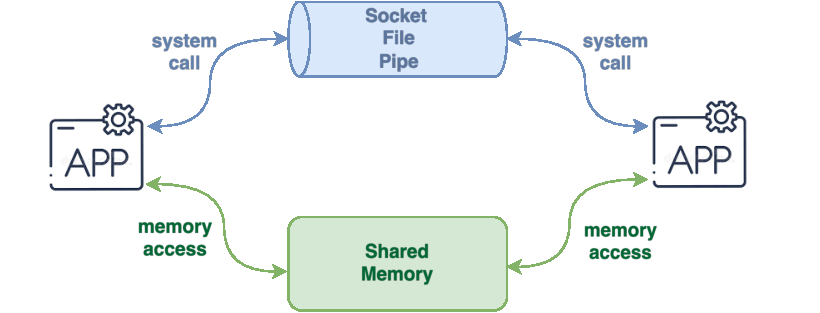
\includegraphics[width=0.7\linewidth]{figures/communication.pdf}
\caption{Applications can communicate through OS interfaces using system calls, or through shared memory using memory accesses. Pipes, files, and shared memory can only be used for communication on the same machine, while sockets can be used for communication both on the same machine and across different machines.}
\label{fig:communication}
\end{figure}

\subsection{Research topic}
% This part of the proposal includes the overall aim, objectives and background. It also deals with the scientific originality and/or the innovative approach of the proposed research and investment, including its cutting-edge aspects and/or groundbreaking character. 


The transition to quantum-resistant cryptography is an urgent European and Dutch priority, reflected in the EU's coordinated roadmap, the Dutch NCSC's guidance, and the joint AIVD, CWI, and TNO migration handbook~\cite{EC2025PQCTransition,NCSCQuantumSafeGuidance,AIVDCWITNO2024Handbook}. Expert discussions of post-quantum security also emphasize the need to begin migration early and the risks of delayed adoption~\cite{Preneel2025QuantumSafeMigration,Preneel2026RiskOfBeingLate}. The EU roadmap calls for Member States to begin transitioning by the end of 2026 and for critical infrastructure protection to migrate by the end of 2030~\cite{EC2025PQCTransition}. Preparing existing systems is particularly challenging: the AIVD highlights long-lived systems that are difficult or impossible to update and warns that migration can take many years~\cite{AIVD2026QuantumThreat}, while ENISA identifies protocol-integration challenges that extend beyond replacing cryptographic algorithms~\cite{ENISA2022PQCIntegration}, motivating practical ways to retrofit quantum-resistant protection.

\medskip

Applications can communicate using various methods: sockets, shared memory, pipes, and files, as illustrated in Figure~\ref{fig:communication}. For communication across different machines, applications use sockets, which create a communication channel between the different hosts; both ends of the communication then use system calls, requests that an application makes to the operating system kernel, to send and receive data through this channel. Once applications reside on the same physical machine, they can also use sockets, or other system call-based techniques such as pipes and files, to communicate with each other. However, shared memory is the dominant communication method on the same machine, owing to its efficiency: it only requires memory accesses, whereas system call-based techniques are used only as a backup or by legacy applications~\cite{Volckaert2016ReMon}.

\medskip

Rewriting applications to support quantum-resistant communication is, of course, an option, but it is not always feasible. Legacy software is often only available as a compiled executable, without access to its source code, which rules out this option entirely; government reports in both the United States and the Netherlands describe how such legacy systems, some running decades-old languages such as COBOL on unsupported hardware and software, remain in critical use across public administration and are difficult or costly to replace~\cite{GAO2025LegacySystems,AcICT2025Legacy}. Even when the source code is available, modifying it is time-consuming and error-prone, as changes to long-lived, poorly documented codebases can introduce subtle regressions. These constraints motivate solutions that can facilitate the migration to quantum-resistant communication without requiring applications to be rewritten.

\medskip

Existing solutions provide only partial answers to this challenge. Security gateways act as intermediaries that wrap an application's existing network connections in a protective tunnel, for instance using TLS, without requiring any changes to the application itself~\cite{Durumeric2017HTTPSInterception,Stunnel2026Manual}. However, they do not encrypt the segment between the application and the gateway, in either direction, since this segment is typically assumed to run over a trusted local network, and, operating purely at the network level, they do not cover local communication on the same machine, such as shared memory, pipes, and files. IPsec protects network traffic at the IP layer by authenticating and encrypting packets exchanged between hosts~\cite{Kent2005RFC4301}, but its inherent complexity has limited interoperability across implementations~\cite{Pepelnjak2013IPsecComplexity}, and it requires a compatible implementation and sufficient configuration privileges at both communicating endpoints, which is not available everywhere and makes adoption challenging in practice; like security gateways, it also does not cover local communication, including shared memory, pipes, and files. VM-based solutions run applications inside confidential virtual machines and can, in principle, protect both local communication, including shared memory within the virtual machine boundary, and network communication, for example by automatically wrapping traffic in mutual TLS~\cite{Misono2024ConfidentialVMs,EdgelessContrast2026}. However, such solutions typically require specialized confidential-computing hardware or changes to how applications are deployed, and the added virtualization, attestation, and encryption layers introduce significant performance overhead.

\medskip

On-TRAQ's central idea is to build a security layer that interposes all communication between applications, regardless of whether the communicating applications reside on the same machine or on different machines. The key observation is that, regardless of the specific communication method used, data ultimately passes through memory: system calls exchange data through memory buffers supplied by the application, for instance when sending or receiving over a socket, pipe, or file, while shared memory communication accesses a memory region directly. On-TRAQ therefore proposes to interpose both on system calls and on accesses to shared memory, and to insert a post-quantum protection layer at these interposition points. Data leaving an application is then transparently encrypted before being written to the corresponding channel, and data arriving at an application is transparently decrypted before being delivered to it, without requiring changes to the communicating applications themselves.

\medskip

Existing interposition solutions come with limitations. In this paragraph, we discuss the main approaches and their trade-offs. Interposition techniques, whether applied to system calls or to memory accesses, have traditionally been implemented through cross-process designs~\cite{Volckaert2013GHUMVEE,StraceManual2026,GdbManual2026}, in which a separate tracer process observes and mediates a target application. Such designs are secure, since process isolation prevents a potentially compromised application from tampering with the interposition logic; however, the frequent context switches required to hand control to the tracer on every intercepted operation introduce substantial performance overhead~\cite{Volckaert2016ReMon,Connor2020PKUPitfalls}. In-process designs avoid this overhead by executing the interposition logic within the application's own address space, typically using binary rewriting. However, such approaches depend on brittle heuristics~\cite{Yasukata2023Zpoline,Jacobs2024LazypolineSyscall} or representative inputs~\cite{Gomez2025ClairObscur}, and, because the interposition logic runs in the same address space as the application, a compromised application can, in principle, tamper with or bypass it entirely. Other approaches instead rely on intrusive modifications such as changes to the operating system or the underlying hardware~\cite{Schrammel2022Jenny,Schrammel2020Donky,Hedayati2019Hodor}, or custom libOS/libc environments~\cite{Yang2024Endokernel}; while such modifications can improve performance or strengthen security, they do so at the cost of increased deployment complexity, reduced portability, and an expanded trusted computing base (TCB).

\medskip

On-TRAQ's aim is to build a practical approach for secure and efficient retrofitting. We focus closely on potential usability, security, and performance side-effects, since such issues usually make the adoption of solutions harder. Some performance degradation from the post-quantum cryptographic operations themselves is inevitable and expected; On-TRAQ's goal is to ensure that the interposition mechanism itself does not introduce additional overhead beyond this unavoidable cost.

\medskip

On-TRAQ is therefore guided by a central research question:

\begin{center}
\textit{``Can we transparently retrofit quantum-resistant communication security \\ into existing applications using an interposition-based approach?''}
\end{center}

\av{the comments below may be for the approach but we will see}

\av{na valeis se kedriki thesi to diagramma pou na min afinei amfivolia gia to pou tha einai i lysi sou}

\av{Hybrid blah blah approach … for mgiration according to Kostas}

\av{Start of initialization of connection or shared memory we make the new layer …}

% Table commented out at Alexios's request, kept for reference.
\iffalse
% Add references to representative systems when developing the surrounding discussion.
\begin{table}[htbp]
\centering
\caption{Communication coverage, deployment requirements, and potential performance costs of existing approaches. Coverage depends on configuration and the protection boundary; performance costs require evaluation for specific systems.}
\label{tab:existing-approaches}
\begin{tabular}{@{}p{0.18\linewidth}p{0.15\linewidth}p{0.15\linewidth}p{\dimexpr0.52\linewidth-6\tabcolsep\relax}@{}}
\hline
\textbf{Approach} & \textbf{Shared memory traffic} & \textbf{Network traffic} & \textbf{Outstanding issues} \\
\hline
% Includes proxy-based service meshes; explain their identity and management features in the text.
Security gateways & No & Yes & No coverage of app-to-endpoint and endpoint-to-app traffic \\
\hline
IPsec & No & Yes & Not supported everywhere \\
\hline
VM-based solutions & Yes & Yes & Virtualization cost, platform-specific hardware and runtime requirements \\
\hline
\end{tabular}
\end{table}
\fi

\subsection{Approach}
% Describe which methods and techniques will be used in the proposed research and discuss their applicability and accessibility. Include a detailed work plan and indicate the duration of the proposed research.

\av{Hardware and binary rewriting agnostic ...}

\subsection{Justification}
% Discuss the choice for the type of personnel (PhD or post-doc) and possibly non-scientific staff. Refrain from giving the name of the intended personnel in so far as you already have a candidate in mind.
% Discuss and motivate your choices for budget decisions. 
% Provide a justification for the budget for knowledge utilization.
% Provide a specification and justification for investment costs.
% When filling out the budget table be aware of the following: 
% * Open Access publishing costs should be included under ‘Materials’;
% * Travel and accommodations costs for the scientific position applied for should be included under ‘Materials’;
% * Budget for ‘Scientific personnel at a research organisation abroad’ is not possible in an M-1 application (please see M-2 application form for options). 



\subsection{Embedding of research and relevant expertise of researchers involved}
% Describe how the proposed research fits with the participating researcher(s) and indicate how the proposed research fits within the (inter)national science landscape. Note that referees and the committee do not assess the CV of the applicant but only the extent to which the appropriate expertise of the researchers is involved as well as appropriate embedding of the research and access to the equipment needed. If applicable, you may wish to use the suggested headings. 

Expertise
% Describe the expertise of the applicant, but refrain from including an extensive CV. Hence, you are instructed to only list relevant information regarding expertise without describing a full track record. 
% * You may describe ongoing work and include references to publications showing previous work. Please be consistent in using the same reference format throughout the proposal, i.e. do not highlight your own work in the running text by using bolt font. 
% * Lists or total numbers of prizes, grants, total acquired sum of funding or publications are not allowed. It is allowed to mention specific grants and prizes that are relevant to the project. However, when mentioning such grants, please provide context why the grant is relevant for your proposed project by describing how the current proposal follows up on previous work, how there is synergy between the current proposal and ongoing project(s)/programme(s) or how the network of another programme is relevant to the current proposal.
% Remember to comply with DORA, i.e. do not use quality indicators that are measured on the author or journal level (for more information on DORA see p.1).


%If applicable
Collaborators
%Describe how the proposed research will benefit from local, national and/or international collaborations. Note that the committee will not assess the quality of the collaborations, but assesses if the appropriate embedding of the research and access to the equipment needed is given. Therefore, please refrain from referring to reputation of the collaborators, e.g. do not mention terms as ‘leading institution’ or ‘world renowned scholar’, but instead provide substantiation of relevant qualities and expertise that will benefit the research. You may include references to joint publications with collaborators, to show a successful past/ongoing collaboration. However, be consistent in using the same reference format throughout the proposal.

%If applicable
Infrastructure
%Describe how you have access to the required equipment locally or to larger national or international infrastructures; this may also include digital infrastructure such as access to computational resources or databases.


\subsection{Risk assessment}
% Discuss feasibility of the research proposal and indicate the possible risks involved with the proposed research, including risks from the methods, techniques, available infrastructure, etc. Indicate how these risks can be mitigated and whether an alternative approach (plan B) exists.

\newpage
\section{Scientific and/or societal impact}
% Section A.3 is limited to one page, including figures and tables and excluding literature references. 

% Do not remove the two sentences below and select the chosen impact focus.  
Applicants in the Open Competition Domain Science – M can choose to put primary focus on scientific impact, societal impact, or a combination thereof. This proposal focusses on %Choose from: Primary focus on scientific impact; Comparable focus on scientific and societal impact; Primary focus on societal impact.


% Explanatory Notes
% Select which kind of impact the proposal focusses on and motivate your choice. The applicant has the choice to focus on achieving scientific impact, societal impact, or a combination thereof. It is not necessary to include both types of impact to get a good score for this assessment criterion. A focus on scientific impact, a focus on societal impact, or a combination thereof, can lead to a good score, provided that it is well motivated. However, when focussing on one type of impact, also state how proportional attention will be given to increasing (unforeseen) opportunities for the other type of impact. So, please motivate your choice and elaborate on all applicable parts of the criteria for the chosen form of impact (see call for proposals, section 4.1 Criteria).

%Scientific impact is the broadening or deepening of one's own or other scientific fields through new knowledge and/or expertise. The potential and relevance of research results for one’s own discipline and related discipline(s) and the potential and relevance of the research results for the wider scientific field form part of the assessment when a focus on scientific impact or a cohe assessment when a focus on societal impact or a comparablemparable focus for both scientific and societal impact is chosen.

%Societal impact here stands for changes that (partly) result from knowledge and skills generated by this research. These changes contribute to the well-being of people, planet and society for this and future generations. The potential for societal impact in the short and long term and the vision of the way(s) in which the proposed research could lead to societal impact form part of t focus for both scientific and societal impact is chosen.


\newpage
\section{Literature/references (in this proposal)}
% The list of references should be relevant to the research proposal, cited in the texts of sections A.2 and A.3. Be consistent in using the same reference format throughout the proposal and only include 'open literature'. It should not include internal documents (such as master theses) nor should it be a mere list of publications of the main applicant. If possible, you are strongly encouraged to include a DOI. This section does not count toward the page limitations.


% EXAMPLE: Using bibtex
\bibliographystyle{unsrtnat-nolabel}
\begingroup
\raggedright
\bibliography{application}
\endgroup

% EXAMPLE: Using thebibliography
%\begingroup % KEEP THIS
%\renewcommand{\section}[2]{} % KEEP THIS
%\begin{thebibliography}{99} % 99 is the maximum # of entries for LaTeX
%\bibitem{1979_Adams}
%  Douglas Adams. \textit{The Hitchhiker's Guide to the Galaxy}. London, UK, 1979.
%
%\bibitem{1905_Einstein}
%  Albert Einstein. {\"U}ber die von der molekularkinetischen Theorie der W{\"a}rme geforderte Bewegung von in ruhenden Fl{\"u}ssigkeiten suspendierten Teilchen. \textit{Ann. Phys.}, 17:549-560, 1905.
%
%\end{thebibliography}
%\endgroup % KEEP THIS


%%%%%%%%%%%%%%%%%%%%%%%%%%%%%

\part{Applicant and additional information}

\section{NWO Scientific Classifications (disciplines)}
% Include at least one and at most five NWO scientific classifications (disciplines) applicable to your research proposal. The list of admissible disciplines can be found in section 7.1 of the call for proposals, round 2026-2027. Please indicate for each chosen disciplines (in percentages) the relevance to your research proposal. Use increments of 5%. The minimum percentage can be 20% and the sum of percentages should not exceed 100%. 
%The disciplines correspond to the discipline codes asked for when submitting your proposal through NWO's online application system ISAAC and should be stated there as well. The disciplines indicated in the application are used by the ENW office to distribute the submitted applications across the cluster committees.
% Please adjust the table accordingly.

\begin{tabular}{ p{3cm} p{3cm} p{3cm} p{3cm}  }
 Disipline 1:   &     & Weight: &   \\
 %Optional: Discipline 2: &    &  Weight:   &\\
 %Optional: Discipline 3: &  & Weight: &  \\
 %Optional: Discipline 4:    & & Weight: &  \\
%Optional: Discipline 5: &   & Weight: &\\

\end{tabular}


\section{Main applicant - additional information}
% NWO corresponds with you via email. Please, make sure that your email address at work is listed correctly in your profile in ISAAC. Tip: check your spam filter regularly as it might happen that an NWO email ends up there. NWO accepts no liability in case emails end up in the spam filter/box.

% This is new table environment with only two columns, whose width can be specified
\begin{texttable}{8cm}{9cm}
  Name (titles, initials, first name, last name): & \\ % Prof. dr. J. (Joan) Doe
  Affiliation - university/institute: & \\ % University of Discworld
  Affiliation - department: & \\ %Department of Magic
  Position: & \\ % Choose: professor / associate professor / assistant professor / other (specify)
  Paid position: & \\ % Choose: yes / no
  Type of contract: & \\ % Choose: tenure track / permanent / probationary one or two year contract
  End date of contract: & \\ % Fill out: N/A or dd-mm-yyyy (provide a statement on guidance when your contract does not cover the runtime of the project in case of tenure track or probationary contract or upcoming retirement)
\end{texttable}

\section{Other pending or future grant applications on the same research topic}
Yes/no
% If yes, please indicate below each proposal on the same research topic as the current proposal (to be) submitted to NWO or other funding agencies by you or by members of your research group. Describe the difference (give a percentage) of the current proposal with the other proposals. Running grants do not need to be reported. Please bear in mind that NWO does not fund the same/similar research twice. Copy and paste the table as often as needed.

% This is new table environment with only two columns, whose width can be specified
\begin{texttable}{8cm}{9cm}
  Title proposal: & \\ % The answer to life, the universe and everything
  Applicant(s): & \\ % prof.dr. J. (Joan) Doe
  Funding agency and call: & \\ % ERC, Starting Grant
  Budget applied for: & \\ % k� 1.200
  Date of submission: & \\ % 1 August 2022
  Estimated date of decision: & \\ % 1 May 2023
  Difference with this proposal: & \\ % 75% difference
  Describe difference: & \\ % Instead of using Deep Thought we will ask the mice
\end{texttable}


\section{Public summaries} % Also needs to be uploaded in ISAAC
% Include a short (max. 100 words) public summary both in Dutch AND in English with a catchy title, which NWO can use in press releases and on their website in case your research proposal gets granted.

Dutch title and summary

English title and summary

\section{Questions Data management section}
% Explanatory Notes
% Responsible data management is part of good research. To promote effective and efficient data management,  data sharing and data reuse, NWO expects researchers to carefully manage data resulting from NWO-funded research and prospectively plan for which data will be preserved and shared.

% With the data management section, NWO mainly wants to raise awareness about the importance of responsible data management. The section is therefore not included in a committee's decision about whether or not a proposal should be awarded funding. NWO does, however, submit this section to the committee and referees for advice. 

% It is recommended that you seek advice from a data steward or research support office at your home institution to complete this section. They will be able to recommend suitable storage facilities and repositories for your data, and to advise on data management costs. After a proposal has been awarded funding, grantees are required to elaborate the data management section into a detailed data management plan explaining how research data and other results emerging from the NWO-funded research will be stored and made findable, accessible, interoperable and reusable (FAIR). 

% What does NWO understand as research data?
% Research data are the evidence that underpin the answer to research questions, and can be used to validate findings. Data can be quantitative information or qualitative statements collected by researchers in the course of their work by experimentation, observation, modelling, interview or other methods, or information derived from existing evidence. For the purpose of NWO's data management policy, the definition of research data does not include physical objects such as scientific and archaeological collections, physical arts works or biobanks; however, digital information extracted from such objects are to be regarded as research data. Software is also not included in the definition of research data. NWO recognizes that software (algorithms, scripts and code developed by researchers in the course of their work) may be necessary to access and interpret data. In such cases, the data management plan will be expected to address how information about such items will be made available.

% What data does NWO expects you share and preserve?
% Research results should be stored in such a way that they can be retrieved and reused in the long term, also by researchers in disciplines and organisations other than those in which the research took place. The operating principle is that all stored data are, in principle, freely accessible and that access is only limited if needed for reasons such as privacy, public security, ethical restrictions, property rights and commercial interests. 
% NWO expects researchers to preserve the data resulting from their projects for at least ten years, unless legal provisions or discipline-specific guidelines dictate otherwise. As much as possible, research data should be made publicly available for reuse, unless there are valid reasons not to do so. As a minimum, NWO requires that the data underpinning research papers should be made available at the time of the article's publication. Any tools or software (algorithms, scripts and code developed by researchers in the course of their work) necessary to access and interpret data should be made available alongside the data.

% The costs of data management are eligible for funding and should be included in the project budget. 
% Important factors that determine the costs are: 
% * the type of data; 
% * the capacity needed for storage and backup; 
% * the amount of work needed to allocate metadata and the compilation of other documentation such as codebooks and the queries used in the statistical package; 
% * the extent to which the data needs to be protected; 
% * the hiring in of external data management expertise or other expertise.


\begin{enumerate}[align=left,labelindent=0pt,labelsep=!,itemindent=0pt,labelwidth=1em]
\item Will this project involve re-using existing research data?\\ % to check box use $\boxtimes$
$\square$ Yes: From my own or a collaborator's prior research.\\ % to check box use $\boxtimes$
$\square$ Yes: Publicly available data.\\ % to check box use $\boxtimes$
$\square$ No: Have you considered re-using existing data but discarded the possibility? Why? % to check box use $\boxtimes$
% If no, please briefly explain why; if yes, state any constraints on re-use of existing data if there are any.  

\item Will data be collected or generated that are suitable for reuse? \\ % to check box use $\boxtimes$
$\square$ Yes: Please answer questions 3 and 4.\\ % to check box use $\boxtimes$
$\square$ No: Please explain why the research will not result in reusable data or in data that cannot be stored or data that for other reasons are not relevant for reuse. 

\item After the project has been completed, how will the data be stored for the long-term and made available for the use by third parties? Are there possible restrictions to data sharing or embargo reasons? Please state these here.


\item Will any costs (financial and time) related to data management and sharing/preservation be incurred?\\ % to check box use $\boxtimes$
$\square$ Yes: Then please be sure to specify the associated expenses as ‘implementation cost’ within the budget post ‘Material costs’ in the budget table of this proposal.\\ % to check box use $\boxtimes$
$\square$ No: All the necessary resources (financial and time) to store and prepare data for sharing/preservation are or will be available at no extra cost. % to check box use $\boxtimes$

\end{enumerate}





% And we're done
\end{document}
